%-----------------------------------------------------------------------------------------------------------------
\chapter[Aplicação do protótipo aos serviços da empresa]{Aplicação do protótipo aos serviços da empresa}
\label{Ch:ServicoExemplo}
\section{Serviço de Gestão de tarefas}

\hspace{1cm}Para evidenciar os benefícios da utilização do \textbf{Docker} na orquestração de serviços foi criado um serviço de gestão de tarefas. Este serviço utiliza uma arquitetura base semelhante aquela utilizada pela equipa de desenvolvimento da \textbf{Yugoup} na construção dos serviços quem compõem a plataforma.

\subsubsection{Pré-requisitos}

\begin{itemize}
 \item Microsoft.AspNetCore.App (2.2.0);
 \item Microsoft.AspNetCore.Razor.Design (2.2.0);
 \item Microsoft.EntityFrameworkCore (2.2.4);
 \item Microsoft.EntityFrameworkCore.SqlServer (2.2.4);
 \item Newtonsoft.Json (12.0.2);
 \item Swashbuckle.AspNetCore (4.0.1);
 \item Swashbuckle.AspNetCore.Swagger (1.0.1);
\end{itemize}

\hspace{1cm}Em termos de modelação o serviço de gestão de tarefas tem uma estrutura de dados semelhante à da figura \ref{Fig:Fig85}, com uma tabela \textit{Employee} e outra tabela \textit{Task}. Cada \textit{Employee} pode ter uma ou mais \textit{Tasks} associadas e cada task só pode estar atribuida a um \textit{Employee}.

\begin{figure}[hbt!]
\centering
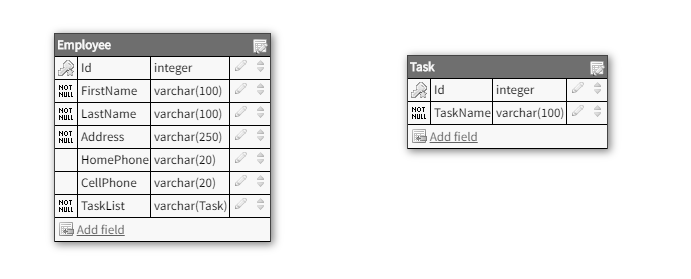
\includegraphics[width=0.7\linewidth]{Cap7/TimeManagement.png}
\caption{Modelo do Serviço de gestão de tarefas}
\label{Fig:Fig85}
\end{figure}

\subsection{Arquitetura da aplicação}

\hspace{1cm}A arquitetura da aplicação não é 100\% idêntica à arquitetura que a empresa utiliza nos serviços da plataforma \textbf{Yugoup}. No entanto, o objetivo não é replicar um serviço com precisamente a mesma arquitetura do serviço \textit{Tenant}. O objetivo é sim publicar um serviço que inclua as camadas de tratamento de dados que a \textbf{Web API} da calculadora não inclui enquanto se aproxima, em termos de complexidade, do nível de desenvolvimento pretendido. A aplicação está organizada em seis \textit{layers} (\ref{Fig:Fig86}): \textbf{Client SDK, Presentation, Application, Domain, Data} e \textbf{Infrastructure} sendo que as camadas \textbf{Client SDK} e \textbf{Infrastructure} não serão utilizadas. É na camada \textbf{Presentation} que estará contida a API do serviço de gestão de tarefas e é a camada de \textbf{Data} vai modelar a base de dados do serviço. As camadas -- \textbf{Application} e \textbf{Domain} -- são o \textit{middleware} entre as camadas de \textbf{Presentation} e \textbf{Data}.

\hspace{1cm}Não será aprofundado o desenvolvimento do serviço em si, nem é esse o objetivo da apresentação deste serviço. Com a construção deste serviço pretende-se demonstrar que, em termos de conceito, o desenvolvimento com \textbf{Docker} pode ser facilmente integrado nas práticas de qualquer empresa de desenvolvimento de software.

\begin{figure}[hbt!]
\centering
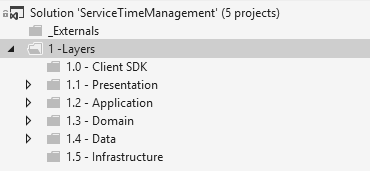
\includegraphics[width=0.5\linewidth]{Cap7/TimeManagementLayers.png}
\caption{Organização do serviço em camadas}
\label{Fig:Fig86}
\end{figure}

\hspace{1cm}Para que possa ser criada uma imagem do \textit{Docker} são necessários os \textit{paths} dos projetos de \textbf{.NET} (\textbf{.csproj}) que compõem a solução. Uma vez que estes projetos estão associados a ficheiros que são utilizados para executar a aplicação, os mesmos terão de estar referenciados algures no \textit{script}. Como se pode ver na figura \ref{Fig:Fig87}, a solução contabiliza um total de cinco destes ficheiros. Os projetos serão utilizados no \textit{Dockerfile}, juntamente com a solução do serviço, para se poder criar uma versão de \textit{Release} da \textbf{Web API} do serviço de gestão de tarefas e assim gerar a versão final de publicação da aplicação.

\begin{figure}[hbt!]
\centering
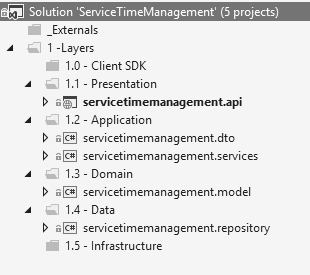
\includegraphics[width=0.4\linewidth]{Cap7/TimeManagementCSPROJ.png}
\caption{Organização dos projetos}
\label{Fig:Fig87}
\end{figure}

\hspace{1cm}A execução da aplicação a partir do ambiente integrado de desenvolvimento é apresentada no \textit{browser} através da interface gráfica do \textbf{Swagger} (\ref{Fig:Fig88}), que é semelhante à apresentaçaõ do serviço \textit{Tenant}, com os métodos da respetiva \textbf{Web API} do serviço de gestão de tarefas. A interface gráfica comunica com o serviço de armazenamento de dados do \textbf{SQL Server} dentro de um \textit{container}. Este método também foi testado no serviço \textit{Tenant}, como poderá ser visto mais à frente. 

\begin{figure}[hbt!]
\centering
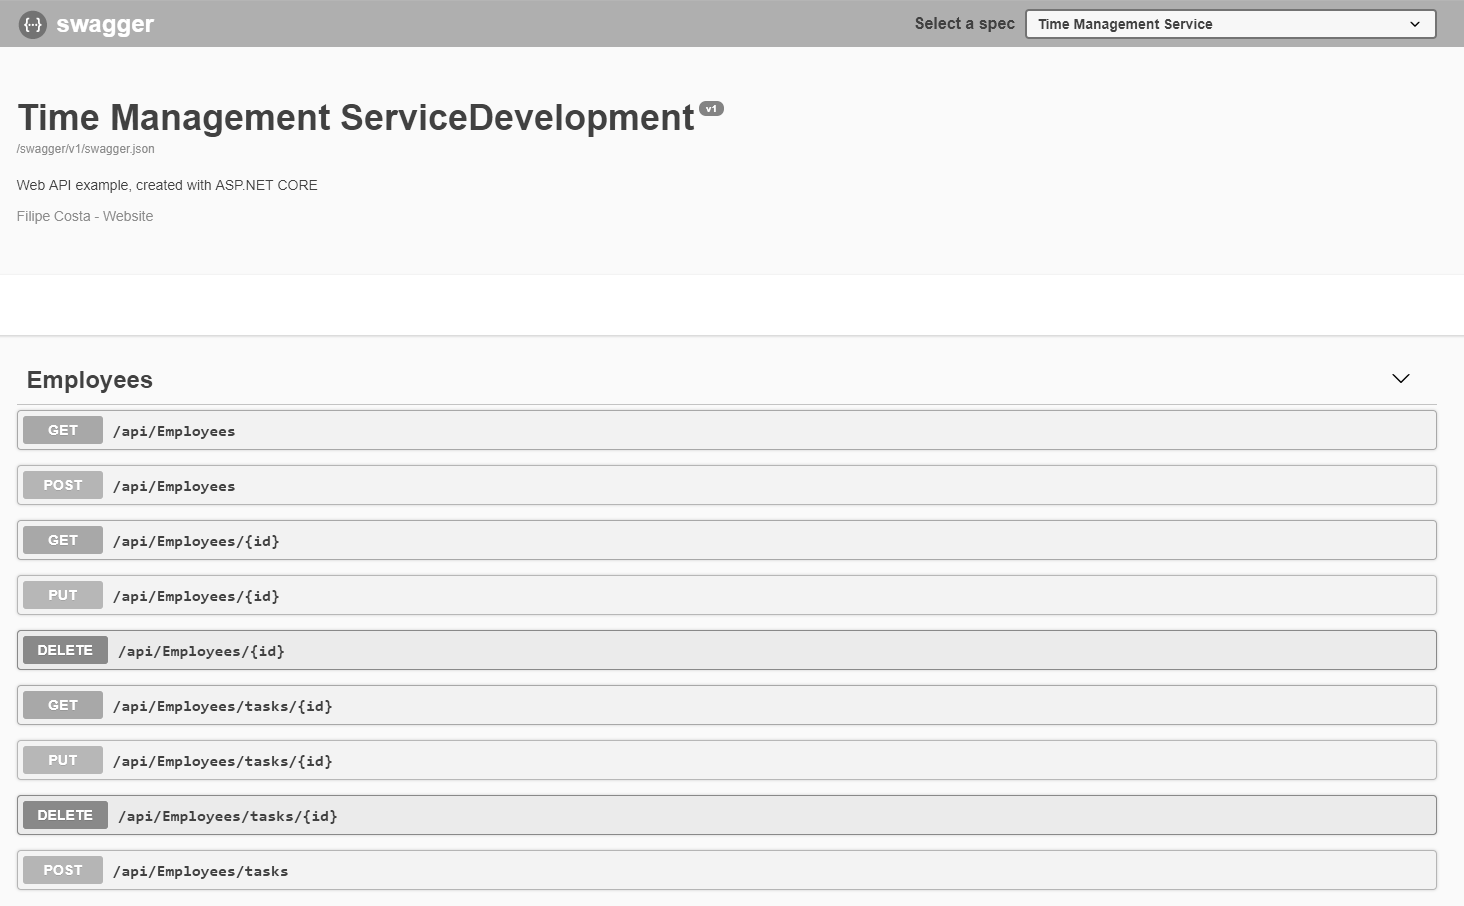
\includegraphics[width=0.8\linewidth]{Cap7/TimeManagementDevelopment.png}
\caption{Interface \textit{Swagger} do serviço de gestão de tarefas}
\label{Fig:Fig88}
\end{figure}

Quando o serviço é inicializado as migrações são feitas para a instância do \textbf{SQL Server} que está a ser executada no \textit{container}, sendo gerada a base de dados \textbf{ServiceTimeManagementContext} com três tabelas (\ref{Fig:Fig89}), \textit{``Employee''}, \textit{``Task''} e \textit{``EFMigrationsHistory''}, a tabela das migrações do \textbf{Entity Framework Core}.

\begin{figure}[hbt!]
\centering
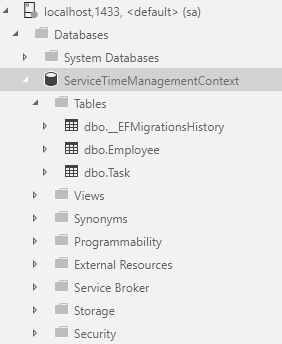
\includegraphics[width=0.35\linewidth]{Cap7/TimeManagementDatabase.png}
\caption{Estrutura da base de dados do \textit{container}}
\label{Fig:Fig89}
\end{figure}

\hspace{1cm}Tal como pode ser visto na figura \ref{Fig:Fig90}, na classe \textit{startup.cs} do serviço de gestão de tarefas, foi adicionado um sufixo ao título da interface gráfica do \textbf{Swagger} com o ambiente atual da aplicação. Neste caso, a aplicação executada a partir do \textbf{IDE} é lançada com as configurações do ambiente de \textbf{Development} (\ref{Fig:Fig88}), \textit{``Time Management ServiceDevelopment''}.

\begin{figure}[hbt!]
\centering
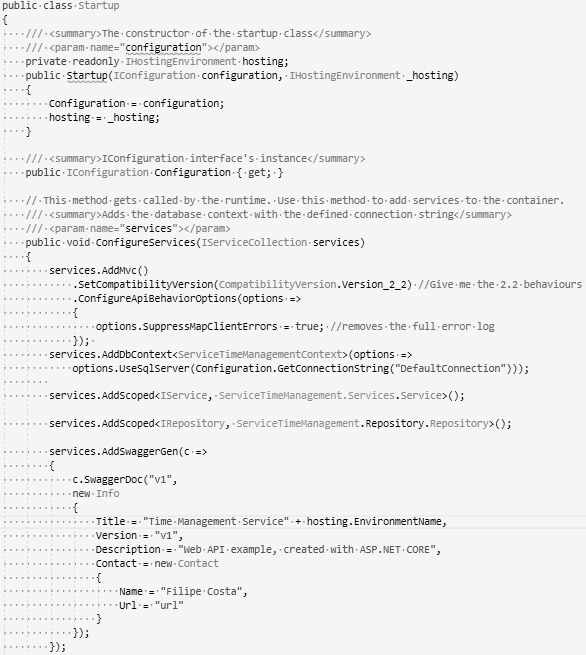
\includegraphics[width=0.9\linewidth]{Cap7/TimeManagementStartupClass.png}
\caption{Estrutura da classe \textit{startup.cs}}
\label{Fig:Fig90}
\end{figure}

\subsection{Criação do \textit{Dockerfile}}

\hspace{1cm}Na criação do \textit{Dockerfile} do serviço foi utilizado o \textit{script} que se pode ver na figura \ref{Fig:Fig91}. A imagem gerada terá a \textbf{tag} do registo seguido do seu nome -- \textbf{localhost:5000/service-time-management} -- e será, mais tarde, publicada no registo privado de imagens.

\begin{figure}[hbt!]
\centering
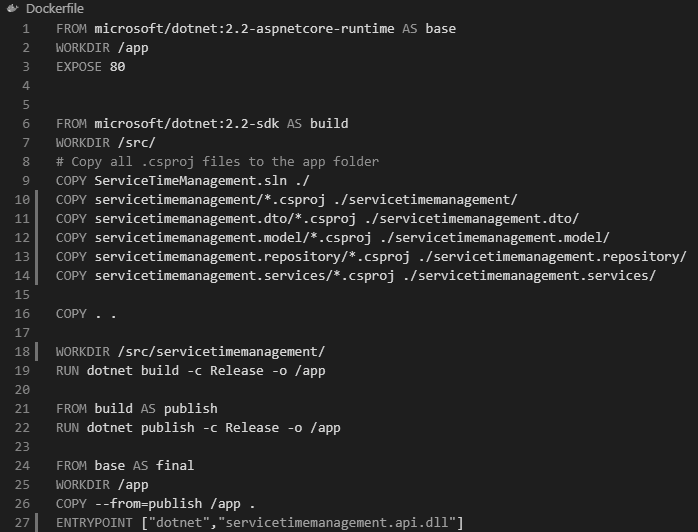
\includegraphics[width=0.95\linewidth]{Cap7/TimeManagementDockerfile.png}
\caption{Estrutura do script de \textit{Docker}}
\label{Fig:Fig91}
\end{figure}

O serviço de gestão de tarefas, depois de publicado, apresenta o sufixo \textbf{Production} junto ao título (\ref{Fig:Fig92}) uma vez que é este o valor que está definido como variável de ambiente para o \textbf{HostingEnvironment} de \textit{Release}. 

\begin{figure}[hbt!]
\centering
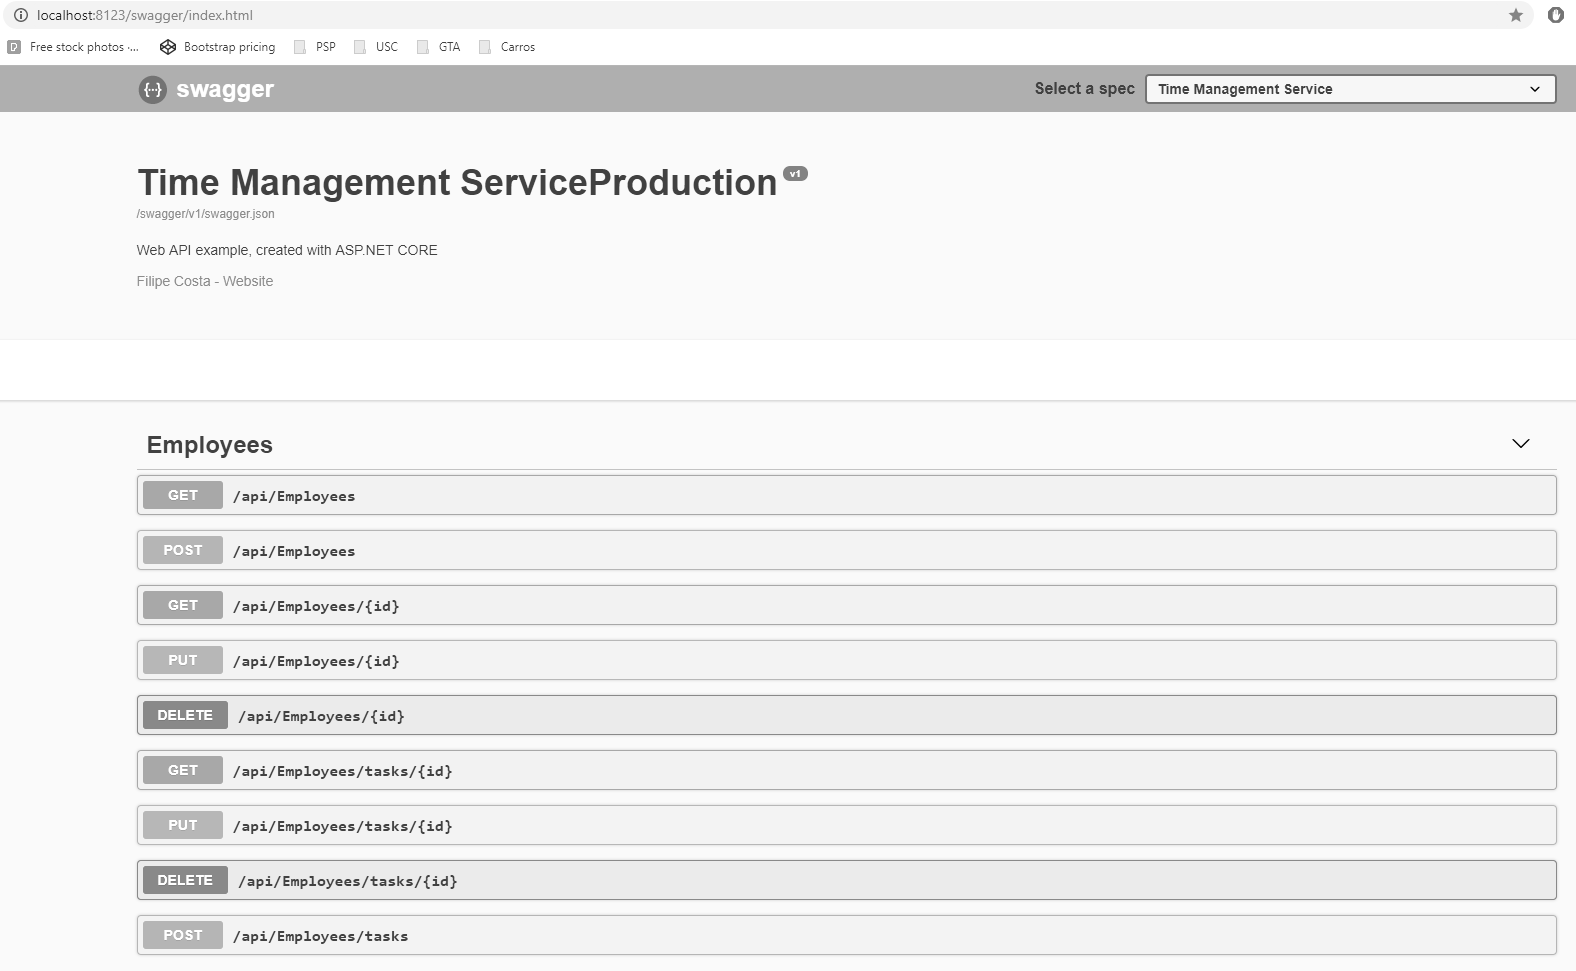
\includegraphics[width=0.9\linewidth]{Cap7/TimeManagementProduction.png}
\caption{Interface \textit{Swagger} do serviço de gestão de tarefa}
\label{Fig:Fig92}
\end{figure}

\subsection{Criação do docker-compose.yml}

\hspace{1cm}A criação de um ficheiro de lançamento da aplicação para \textit{pre-live} vai envolver a execução de quatro \textit{containers}. O primeiro \textit{container} a ser lançado será o da base de dados porque sem ela a aplicação simplesmente não funciona. De seguida são executados dois \textit{containers} com duas aplicações da \textbf{Web API} do serviço de gestão de tarefas, em duas portas diferentes e com \textit{HostingEnvironments} diferentes. Por último lugar, é executado o serviço de \textit{load balancing} da aplicação.

\subsubsection{Serviço de base de dados}

\hspace{1cm}O serviço de base de dados utilizado -- \textbf{MS SQL Server} -- é o primeiro a ser executado e todos os restantes serviços dependem do seu funcionamento. Convém ter em conta que os dois serviços da \textbf{Web API} devem aguardar que a base de dados esteja lançada (\ref{Fig:Fig93}) e devidamente configurada para, só depois, poderem arrancar. Para ultrapassar este problema é necessário garantir que o serviço da \textbf{Web API} só é iniciado depois de ser estabelecida uma conexão ao \textit{container} da base de dados.

\begin{figure}[hbt!]
\centering
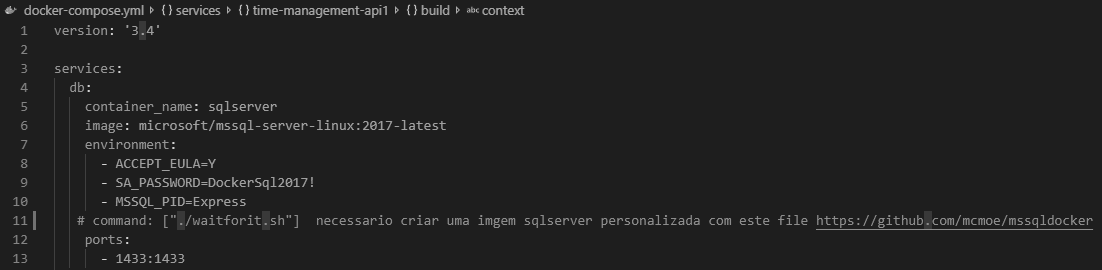
\includegraphics[width=0.9\linewidth]{Cap7/TimeManagementDCSQLServer.png}
\caption{Serviço de base de dados da aplicação}
\label{Fig:Fig93}
\end{figure}

Para este caso a solução passou pela implementação de um ciclo de tentativas de conexão ao serviço de base de dados com recurso a um \textit{try-catch}. Como pode ser visto na figura \ref{Fig:Fig99}, no bloco \textit{try} vai ser utilizado o contexto da base de dados que foi configurado para serem feitas as migrações. Enquanto que na cláusula \textit{catch} é feito um ciclo de 10 tentativas de conexão à base de dados.

\begin{figure}[hbt!]
\centering
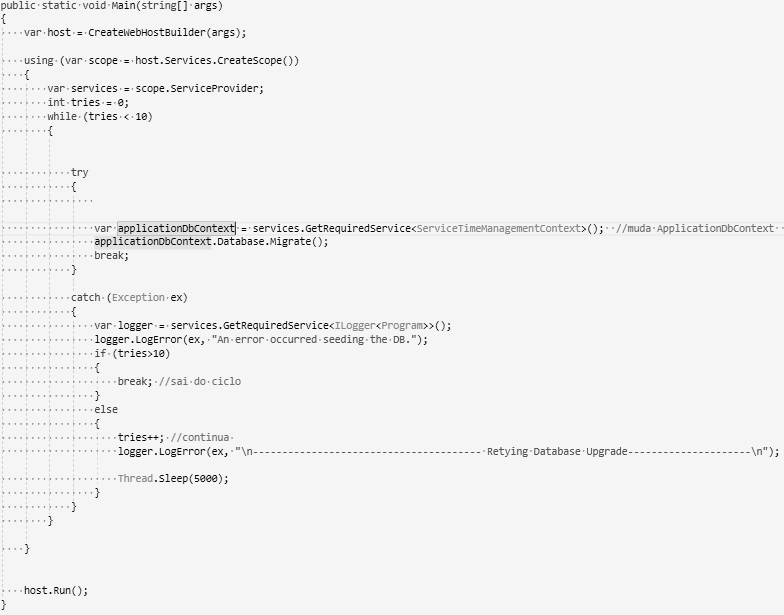
\includegraphics[width=0.9\linewidth]{Cap7/TimeManagementCheckDBService.png}
\caption{Verificação da configuração do Serviço de Base de dados}
\label{Fig:Fig99}
\end{figure}

\subsubsection{Serviço de Web API}

\hspace{1cm}Os dois serviços da \textbf{Web API} dependem do serviço de BD para poderem funcionar. O serviço \textit{time-management-api1} apresenta a variável de ambiente com a configuração de \textit{Release} por defeito. Já o serviço \textit{time-management-api2} apresenta uma variável de ambiente diferente ao utilizador apesar de ter a mesma configuração de \textit{Release} do seu par. Como se pode ver pela figura \ref{Fig:Fig94}, nas variáveis de ambiente \textbf{time-management-api2}, o valor de \textit{HostingEnvironment} daquela instância é definido como \textit{``Test''} através da utilização da variável de ambiente \textbf{ASPNETCORE\_ENVIRONMENT=Test}. Assim sendo, quando for utilizado o \textit{load balancer} para distribuir os pedidos pelas duas \textbf{Web APIs} sabe-se, através do sufixo apresentado no título, qual a instância da API que está a ser apresentada no \textit{browser}. 

\begin{figure}[hbt!]
\centering
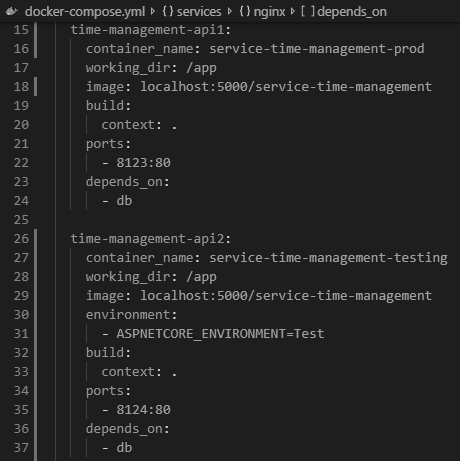
\includegraphics[width=0.45\linewidth]{Cap7/TimeManagentDCWebAPI.png}
\caption{Serviço de apresentação da \textbf{Web API}}
\label{Fig:Fig94}
\end{figure}

\subsubsection{Serviço de \textit{Load Balancing}}

\hspace{1cm}Da mesma forma que os serviços da \textbf{Web API} dependem do serviço de base de dados para poderem ser inicializados, os serviço de \textit{load balancing} vai esperar que as duas APIs estejam lançadas para poder ser executado. Pela figura \ref{Fig:Fig95} pode verificar-se que o \textbf{nginx} é o último serviço a ser executado.

\begin{figure}[hbt!]
\centering
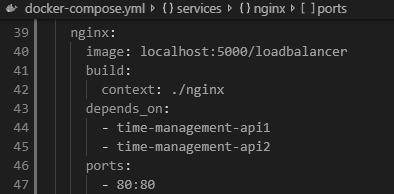
\includegraphics[width=0.45\linewidth]{Cap7/TimeManagementLoadBalancing.png}
\caption{Serviço de \textit{load balancing}}
\label{Fig:Fig95}
\end{figure}

\hspace{1cm}Após a fase de \textit{development}, os passos para a publicação de um serviço repetem-se sistematicamente. A seguir à criação das imagens que vão compor o serviço nas fases de \textit{pre-live} e \textit{production}, é sempre produzido um ficheiro de composição \textbf{(docker-compose.yml)} que vai orquestrar a publicação da aplicação, serviço a serviço, pela sequência cronológica de instruções de publicação que lhe são transmitidas.

\subsection{Considerações}

\hspace{1cm}Este tipo de metodologia de publicação pode ser utilizado localmente ou online, com uma condição. Na máquina onde o serviço é publicado, terá de estar instalado o \textbf{Docker}.

\hspace{1cm}Caso o serviço esteja publicado em rede local, como por exemplo, na máquina de \textit{staging} disponibilizada pela empresa, os custos de operação passam a ser única e exclusivamente a energia consumida pela máquina, contrariamente ao que acontece quando um serviço é publicado online para ser testado. Uma das principais vantagens é a facilidade com que se consegue replicar toda a infra-estrutura, o que facilita não só o desenvolvimento em si, mas também a \textit{pipeline} de teste, porque desta forma é possível criar e destruir os ambientes facilmente.

\hspace{1cm}Um dos contratempos da utilização do \textbf{Docker} (versão do \textbf{Windows}) é a perda de dados em situações como, por exemplo, quando uma máquina é reiniciada sem existir persistência de dados. Estes dados nunca mais serão recuperados, uma vez que por definição os \textit{containers} são voláteis. Assim sendo, para contornar este problema é necessário utilizar \textit{containers} para guardar os dados das aplicações que estão a ser utilizadas, e utilizar os seus volumes como repositórios de dados. Desta forma os dados ficarão sempre persistidos na memória dos outros \textit{containers}, mesmo que o serviço do \textbf{Docker} falhe inesperadamente.

\hspace{1cm}Os próximos passos serão a implementação de uma \textit{pipeline} de integração e entrega contínua para um serviço da plataforma Yugoup. Para tal, será criada uma \textit{branch} paralela à \textit{Master} -- chamada \textbf{cicd} -- que permitirá trabalhar em conformidade com os objetivos estabelecidos pela equipa de orientação sem interferir com os desenvolvimentos da equipa da empresa. O serviço mais importante da plataforma, o \textit{Tenant}, foi o escolhido para percorrer todas as fases de integração contínua.

\section{Plataforma Yugoup}
\label{Ch:Plataforma Yugoup}

\hspace{1cm}A plataforma de comércio eletrónico \textbf{Yugoup} foi desenvolvida segundo o estilo de arquitetura orientada a serviços (por camadas) e contabiliza 36 serviços, no momento de escrita do documento. A arquitetura dos serviços é constituída por 6 camadas -- \textit{top-to-bottom:} \textbf{Client SDK, Presentation, Application, Domain, Data} e \textbf{Infrastructure} -- e inclui testes unitários às camadas de \textbf{Application, Domain} e \textbf{Data}. Para esta fase, o objetivo seria construir uma \textit{pipeline} de testes automatizada. Os desafios seriam a integração de análise estática e o desenvolvimento de testes de integração e performance num serviço disponibilizado, mais concretamente na camada de \textbf{Presentation}. 

\hspace{1cm}A empresa disponibilizou um serviço (\textit{Tenant}) para integração continua numa \textit{pipeline} de testes automatizada com a execução dos testes unitários pré-existentes. Os serviços foram publicados, pela equipa da \textbf{Yugoup} numa máquina, em rede local, dentro do espaço de trabalho o que significa que os testes de integração e performance seriam feitos diretamente contra o serviço \textit{t-yugoup-tenant} publicado em \textit{staging}.

\subsection{Integração contínua do serviço \textit{Tenant}}

\hspace{1cm}Os testes de integração e performance serão desenvolvidos e integrados, juntamente com a análise estática ao código, na instância do \textbf{Jenkins} previamente instalada e configurada na máquina de \textit{staging}.

\subsection{Desenvolvimento dos testes de integração e performance}

\hspace{1cm}Foram desenvolvidos quatro testes de integração e dois testes de performance ao serviço \textit{Tenant}. Como é possível ver na figura \ref{Fig:Fig58}, os testes de integração utilizam uma classe -- \textbf{ClientExtensions} -- cuja função é criar o cliente. Esta classe contém um método -- \textbf{CreateClient} -- que recebe como parâmetro uma \textit{string}. Essa \textit{string} é o \textbf{URL} do serviço do \textit{Tenant} que foi publicado localmente em \textit{staging}.

\begin{figure}[hbt!]
\centering
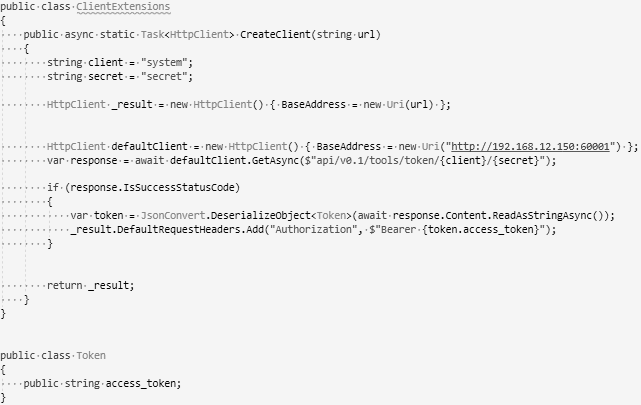
\includegraphics[width=0.9\linewidth]{Cap6/TenantClientExtensions.png}
\caption{Classe \textit{ClientExtensions}}
\label{Fig:Fig58}
\end{figure}

\hspace{1cm}O primeiro teste de integração foi criado para testar a existência do \textbf{GUID} -- \textit{Global Unique Identifier} -- que é gerado automaticamente quando são feitas as migrações, logo após a criação das bases de dados. O cliente gera um \textit{token} de autenticação para o \textbf{Tenant} e as verificações são feitas ao tipo de resposta e ao conteúdo da mensagem (\ref{Fig:Fig59}).

\begin{figure}[hbt!]
\centering
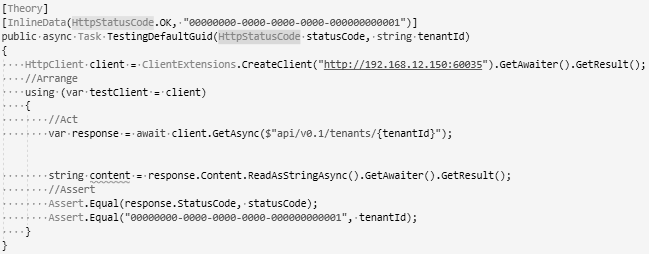
\includegraphics[width=0.9\linewidth]{Cap6/TenantDefaultGUID.png}
\caption{Teste à presença do \textit{Default GUID}}
\label{Fig:Fig59}
\end{figure}

\hspace{1cm}O segundo teste de integração foi criado para testar um GUID inexistente. O cliente gera um \textit{token} de autenticação para o \textbf{Tenant} e as verificações são feitas ao tipo de resposta e ao conteúdo da mensagem (\ref{Fig:Fig60}) à semelhança do teste anterior.

\begin{figure}[hbt!]
\centering
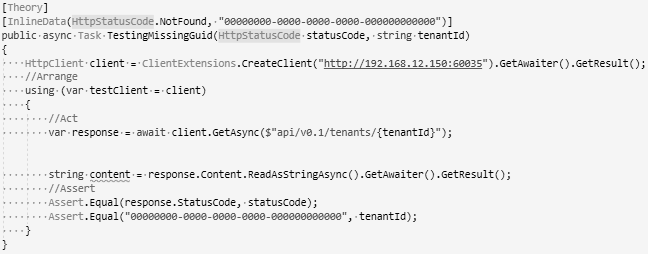
\includegraphics[width=0.9\linewidth]{Cap6/TenantMissingGUID.png}
\caption{Teste à presença de um \textit{GUID} inexistente}
\label{Fig:Fig60}
\end{figure}

\hspace{1cm}O terceiro teste de integração tem uma componente de teste à performance na medida em que é testado o tempo de resposta do pedido de acesso à aplicação com a \textit{property} \textbf{enabled=true} presente na mensagem (\ref{Fig:Fig61}).

\begin{figure}[hbt!]
\centering
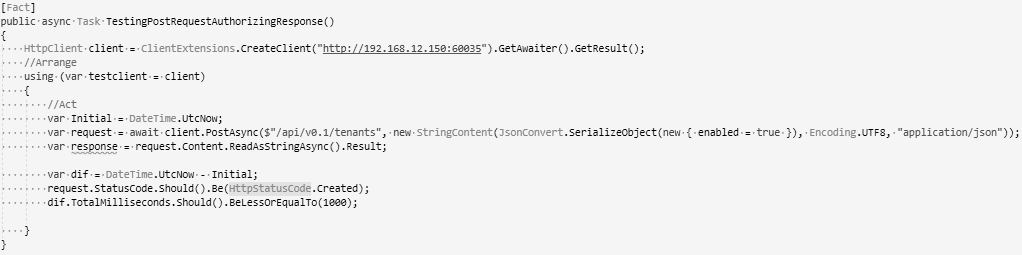
\includegraphics[width=0.9\linewidth]{Cap6/TenantAuthorization.png}
\caption{Teste de acesso autorizado}
\label{Fig:Fig61}
\end{figure}

\hspace{1cm}O quarto teste de integração tem uma componente de teste à performance, semelhante ao teste anterior, na medida em que é testado o tempo de resposta do pedido de acesso à aplicação sem a \textit{property} \textbf{enabled=true} presente na mensagem (\ref{Fig:Fig62}).

\begin{figure}[hbt!]
\centering
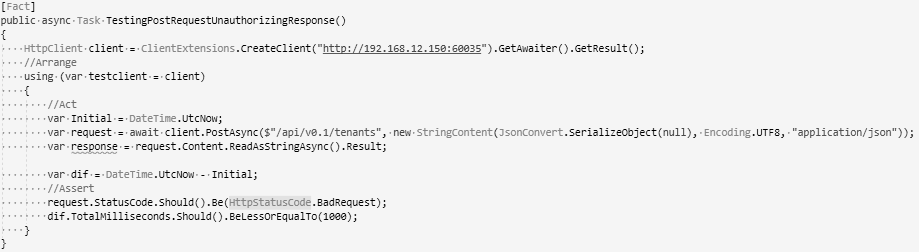
\includegraphics[width=0.9\linewidth]{Cap6/TenantUnauthorized.png}
\caption{Teste de acesso não autorizado}
\label{Fig:Fig62}
\end{figure}

\hspace{1cm}Os testes estão todos organizados de forma a que as \textit{Assertions} sejam feitas ao tipo de resposta esperado, portanto todos os testes foram validados. O próximo desafio é alinhar os testes de integração/performance com todos os testes unitários já existentes. Para tal, na \textit{pipeline} serão necessários todos os serviços com os quais o \textbf{Tenant} comunica.

\subsection{\textit{Pipeline}}

\hspace{1cm}Os serviços da plataforma que estão referenciados no projeto do serviço \textit{t-yugoup-tenant} são necessários para que o projeto possa ser devidamente integrado na \textit{pipeline}. Quer isto dizer que, para que seja possível compilar o código do projeto, seria também necessário integrar na \textit{pipeline} o código de todos os projetos com os quais o \textit{Tenant} tem dependências ou referências. Será portanto necessário gerir vários repositórios e incluir todas as soluções das dependências do projeto numa pasta, que posteriormente será reorganizada, e só depois poderão ser feitas as operações sobre o código. De seguida será então possível integrar análise estática, restaurar as dependências do projeto do serviço \textit{Tenant}, fazer \textit{build} ao projeto, executar testes unitários, testes de integração/performance e, por fim, interpretar os resultados dos testes. Foi também necessário instalar um \textit{plugin} para que se possam analisar vários repositórios em simultâneo.

\hspace{1cm}Para o \textit{setup} do ambiente do \textbf{Jenkins} foi utilizado um \textit{script} semelhante ao da figura \ref{Fig:Fig63}. Este \textit{script} vai criar uma pasta (final) e uma subpasta (src), vai fazer \textit{clone} aos repositórios que fazem parte da plataforma e, por fim, \textit{build} ao projeto. Isto acontece porque, como dito anteriormente, são necessários todos projetos da plataforma \textit{Yugoup}, que estão referenciados no projeto \textit{t-yugoup-tenant}, para que possa ser feita \textit{build} ao serviço da \textbf{Web API} do \textit{Tenant}.

\begin{figure}[hbt!]
\centering
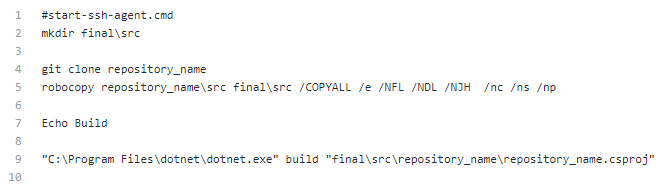
\includegraphics[width=0.9\linewidth]{Cap6/SetupEnvScript.png}
\caption{\textit{Script} de \textit{setup}}
\label{Fig:Fig63}
\end{figure}

\hspace{1cm}No \textbf{Jenkins}, dá-se uma descrição à \textit{pipeline}. Em \textbf{Source Code Management}, selecciona-se o \textit{plugin} \textbf{Multiple SCMs} e configura-se a ligação aos repositórios via \textbf{SSH}. Todos os repositórios que vão ser adicionados à \textit{pipeline} vão seguir a mesma metodologia. Primeiro será inserido o \textbf{URL} do repositório e é seleccionada a credencial de acesso por \textbf{SSH} e só depois é especificada a \textit{branch} sob a qual serão feitas as operações. Por fim, dá-se um nome à pasta onde serão colocados os ficheiros dos projetos (\ref{Fig:Fig64}). As configurações restantes serão idênticas, não existirão \textbf{Build Triggers}, apenas será eliminado o \textit{workspace} antes de cada \textit{build}. 

\hspace{1cm}Em \textbf{Build}, todos os \textit{build steps} utilizados para criar o \textit{setup} serão feitos à semelhança do \textit{script} que se pode visualizar na figura \ref{Fig:Fig63}. À semelhança do \textit{script}, como dito anteriormente, foi criada um diretoria -- final -- e uma subdiretoria -- \textbf{src} -- para onde foram passados os ficheiros dos serviços. Foi utilizado o \textbf{robocopy} para copiar os ficheiros para a subdiretoria: \colorbox{gray}{\textcolor{white}{\$ robocopy project-name folder-path}} juntamente com as opções \colorbox{gray}{\textcolor{white}{/COPYALL /e /NFL /NDL /NJH  /nc /ns /np}} \cite{robocopy}.

\begin{figure}[hbt!]
\centering
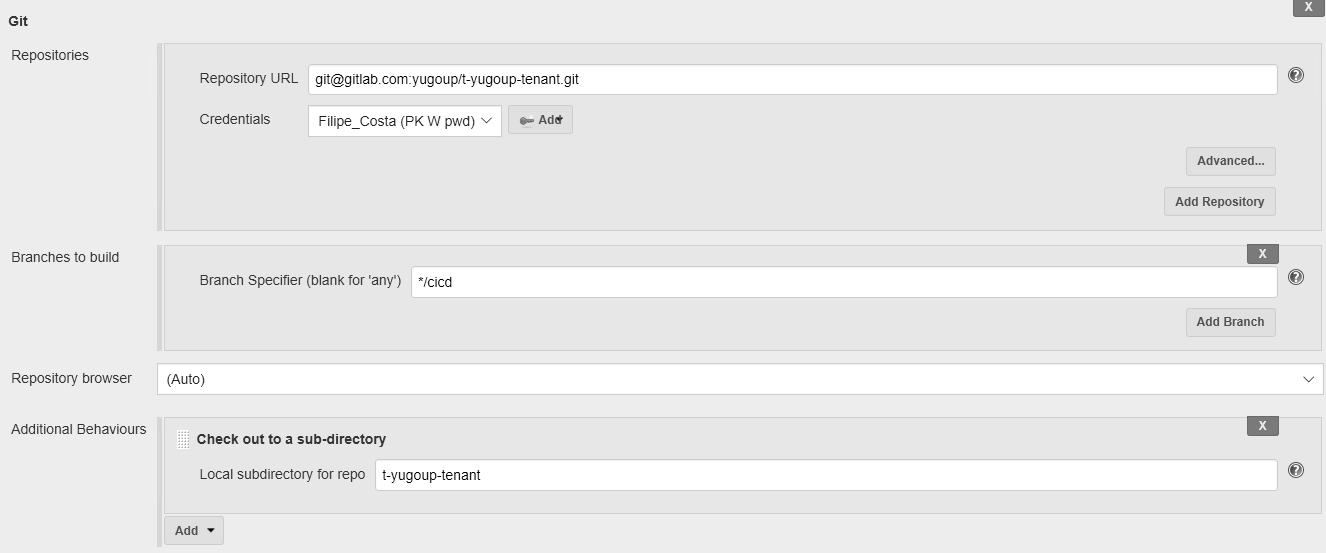
\includegraphics[width=0.9\linewidth]{Cap6/JenkinsMultipleSCM.png}
\caption{\textit{Multiple Source Code Management}}
\label{Fig:Fig64}
\end{figure}

\subsubsection{Fase de \textbf{Build} do projeto}

\hspace{1cm}As primeiras instruções na fase de \textit{build} do projeto \textit{tenant} são a instrução de arranque da análise estática e a instalação dos \textbf{NuGet Packages} presentes num repositório online. Posteriormente é feita \textit{build} à solução do \textit{Tenant} (\ref{Fig:Fig65}).

\begin{figure}[hbt!]
\centering
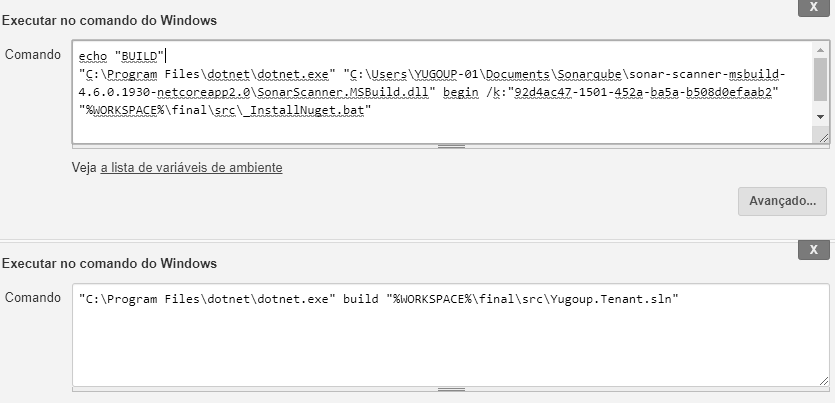
\includegraphics[width=0.9\linewidth]{Cap6/JenkinsTenantBuild.png}
\caption{Análise estática, \textit{Restore} e \textit{Build} }
\label{Fig:Fig65}
\end{figure}

\hspace{1cm}Para iniciar a análise estática foram repetidos os passos do capítulo anterior. Depois de iniciada a análise estática e antes e antes de ser feita \textit{build} à solução é executado um \textit{script} que vai instalar todas as dependências através da utilização de um ficheiro \textbf{batch} (.bat) desenvolvido pela equipa da \textbf{Yugoup}. Na fase de \textit{build} da solução -- e após o \textit{setup} do ambiente -- todas as soluções serão revistas pela análise estática. Isto acontece porque se está a fazer \textit{build} à solução do \textit{Tenant} em conjunto com as soluções das suas dependências.

\subsubsection{\textit{Build} e \textit{Run} dos testes unitários}

\hspace{1cm}Também à semelhança daquilo que foi feito no capítulo anterior, os testes unitários terão de ser compilados (\ref{Fig:Fig66}) e executados (\ref{Fig:Fig67}) para que sejam gerados resultados. Só depois se podem armazenar e apresentar estes resultados. O mesmo acontece com os testes de integração e performance.

\begin{figure}[hbt!]
\centering
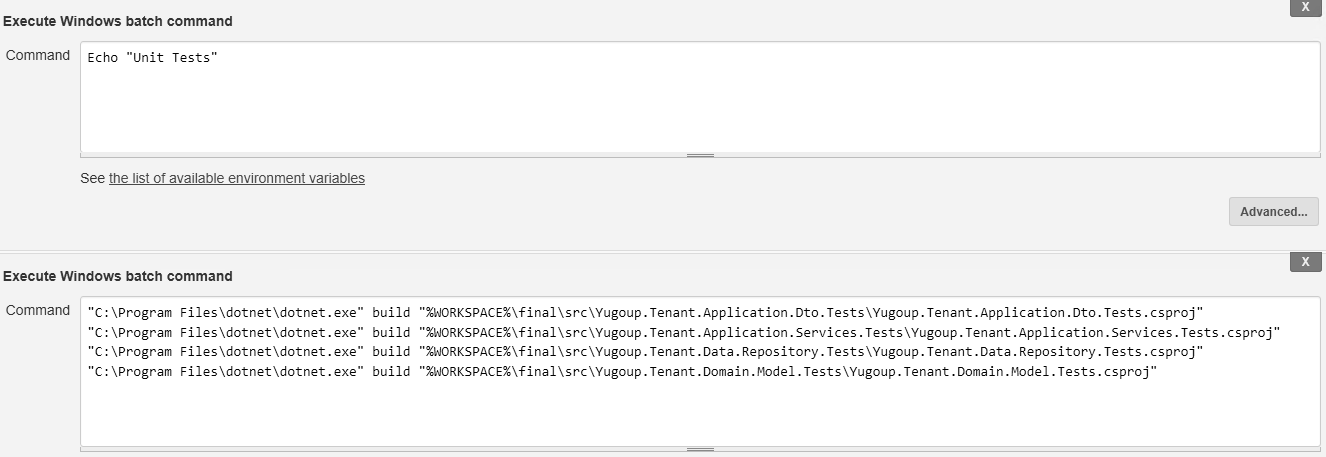
\includegraphics[width=0.9\linewidth]{Cap6/TenantUnitTests.png}
\caption{Compilação dos projetos de teste}
\label{Fig:Fig66}
\end{figure}

\begin{figure}[hbt!]
\centering
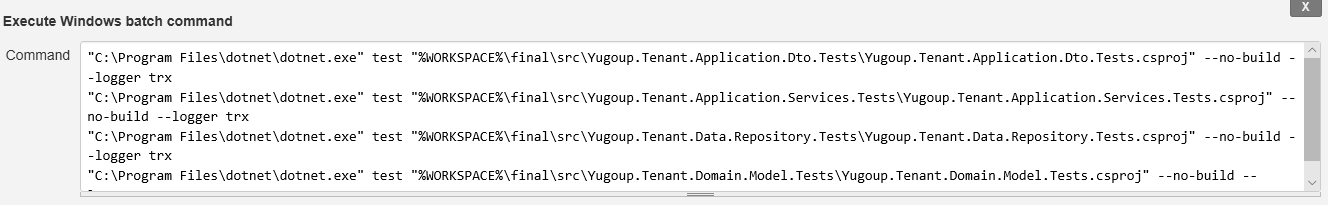
\includegraphics[width=0.9\linewidth]{Cap6/TenantUnitTestsExecution.png}
\caption{Execução dos projetos de teste}
\label{Fig:Fig67}
\end{figure}

 As instruções de execução dos testes já são conhecidas e, como pode ser visto pela figura (\ref{Fig:Fig68}), antes da execução dos testes de integração é necessário executar outro \textit{script}, através de um ficheiro \textbf{batch} (.bat), para remover o \textit{feed} das dependências do projeto. Resta parar a execução da análise estática e pode então proceder-se à execução dos testes de integração e performance.


\begin{figure}[hbt!]
\centering
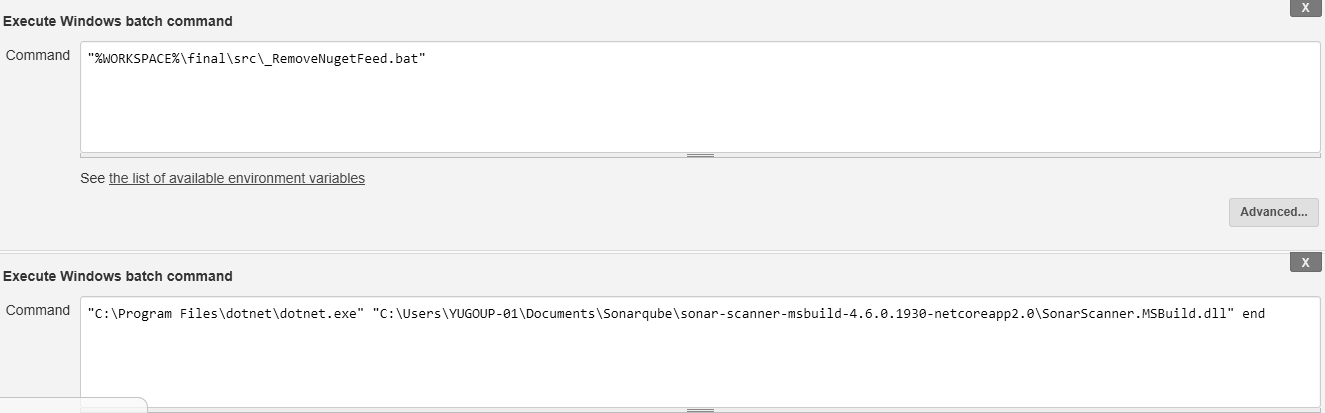
\includegraphics[width=0.9\linewidth]{Cap6/TenantRemoveFeed.png}
\caption{Remoção das dependências}
\label{Fig:Fig68}
\end{figure}

\subsubsection{\textit{Build} e \textit{Run} dos testes integração e performance}

\hspace{1cm}Os testes de integração e performance são compilados e executados (\ref{Fig:Fig69}) à semelhança dos testes unitários. Na fase de \textbf{Post-build Actions} vão interpretar-se os resultados de todos os testes em simultâneo. 

\begin{figure}[hbt!]
\centering
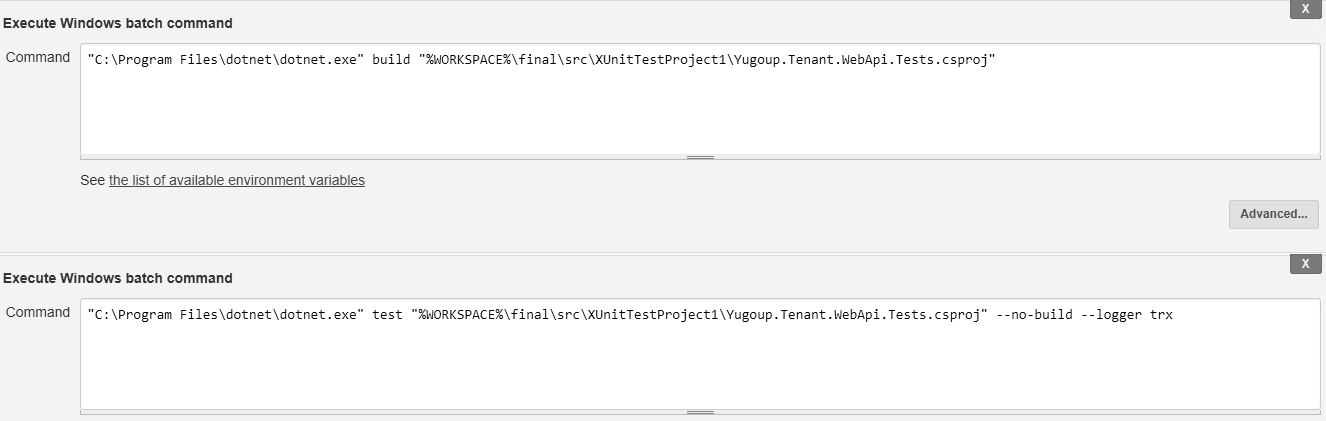
\includegraphics[width=0.9\linewidth]{Cap6/TenantIntegrationTests.png}
\caption{Compilação e execução dos testes de integração e performance}
\label{Fig:Fig69}
\end{figure}

\hspace{1cm}Um complemento interessante à \textit{pipeline} seria a geração automática de uma imagem de \textbf{Docker} do serviço \textbf{t-yugoup-tenant}. A imagem foi gerada e exposta numa porta pública mas o seu processo de geração não foi incluído na \textit{pipeline}. Apesar da aplicação ter sido publicada, o seu endereço não estava autorizado a aceder aos serviços da plataforma Yugoup. Em baixo é apresentada a estrutura do \textit{Dockerfile} que deu origem à imagem do serviço e são delineados um conjunto de \textbf{Next Steps} para o futuro, caso a equipa pretenda integrar na \textit{pipeline} o processo de geração automática da imagem através de um \textit{Dockerfile}.

\subsection{Geração da imagem do serviço \textit{Tenant}}

\hspace{1cm}A versão de \textit{Release} da \textbf{Web API} do serviço \textit{Tenant} sobre a qual estão a ser feitos os testes de integração foi publicada na máquina de \textit{staging} através de \textbf{Web Deploy} \cite{webdeployiis}. Contudo, seria interessante publicar uma imagem de \textbf{Docker} do serviço \textit{Tenant} semelhante à imagem da \textbf{Web API} da Calculadora. 

\hspace{1cm}Foram incluídos todos os projetos (\ref{Fig:Fig77}) que compõem o serviço \textit{Tenant} e foi feito \textit{restore} a partir do repositório de artefactos que foi disponibilizado pela equipa do projeto (\ref{Fig:Fig78}). De seguida foi copiada a pasta de configuração do ficheiro \textbf{NuGet.config} para a pasta \textbf{/app}, foram executadas as intruções de \colorbox{gray}{\textcolor{white}{\$ dotnet build}} e \colorbox{gray}{\textcolor{white}{\$ dotnet publish}} (\ref{Fig:Fig79}) com a configuração de \textit{Staging} e o \textit{output} a ser colocado na pasta \textbf{/app}. Por fim foi publicada a aplicação com a \textit{dynamically linked library} da \textbf{Web API} do serviço de \textit{Tenant} tal como pode ser visto na figura \ref{Fig:Fig79}.

\begin{figure}[hbt!]
\centering
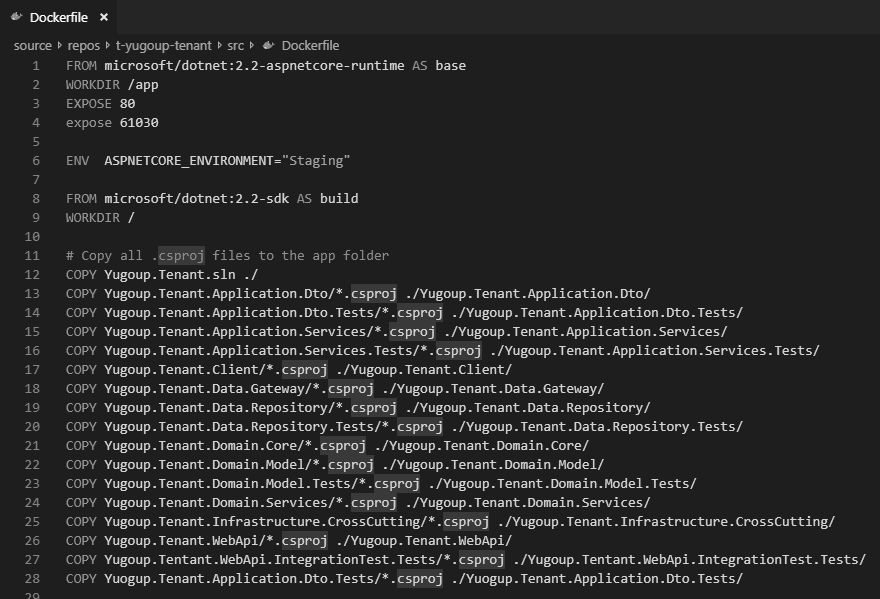
\includegraphics[width=0.9\linewidth]{Cap6/TenantDockerfileCSPROJ.png}
\caption{Dockerfile do serviço \textit{Tenant}}
\label{Fig:Fig77}
\end{figure}


\begin{figure}[hbt!]
\centering
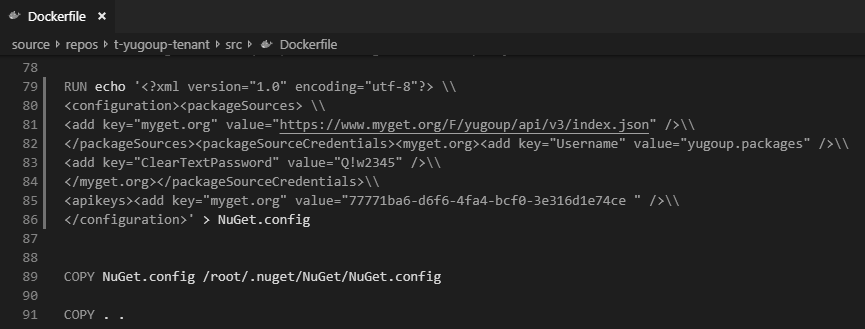
\includegraphics[width=0.9\linewidth]{Cap6/TenantDockerfileNuGetConfig.png}
\caption{Dockerfile do serviço \textit{Tenant}}
\label{Fig:Fig78}
\end{figure}

\begin{figure}[hbt!]
\centering
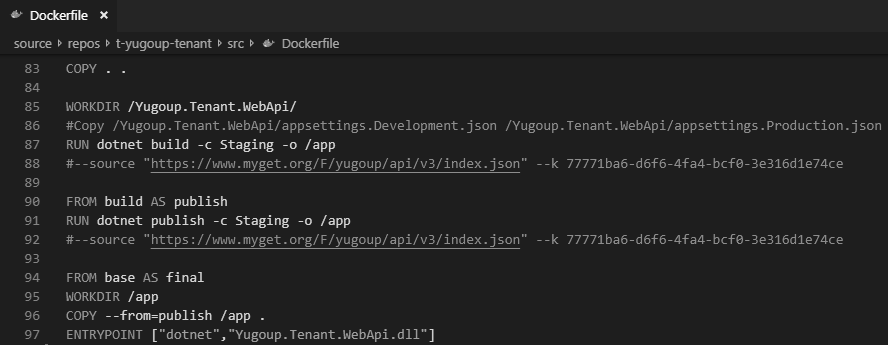
\includegraphics[width=0.9\linewidth]{Cap6/TenantDockerfilePublish.png}
\caption{Dockerfile do serviço \textit{Tenant}}
\label{Fig:Fig79}
\end{figure}

\hspace{1cm}Sem alterar o código da plataforma, uma vez que não eram permitidas alterações à sua base, e sem interferir com os tipos de bases de dados que a plataforma está a utilizar, foi criada uma base de dados do mesmo tipo que o serviço utiliza -- \textbf{SQL Server} -- através do uso de uma imagem de \textbf{Docker} disponibilizada no repositório oficial que a \textbf{Microsoft} criou para imagens do \textbf{Microsoft SQL Server} \cite{dockersqlserver}. Também é necessário fazer uma pequena alteração à \textit{connection string} do serviço \textit{Tenant} uma vez que terá de ser ligeiramente diferente daquela que o serviço que está publicado na máquina de \textit{staging} utiliza atualmente para que a base de dados a ser executada dentro de um \textit{container} possa ser acedida e manipulada. 

    \hspace{1cm}Tal como é apresentado na figura \ref{Fig:Fig80}, pode ser vista a \textit{connection string} de ligação ao \textit{container} do \textbf{Docker} onde está a ser executada a imagem do \textbf{SQL Server}. Comentada, na linha anterior, também pode ser vista a \textit{string} de ligação à base de dados antiga. Para verificar que a base de dados de \textbf{SQL Server está a funcionar} é necessário aceder ao \textit{container} via \textbf{Azure Data Studio}. São assim necessárias as credenciais de acesso com as quais foi lançado o serviço de base de dados e é necessário colocar no campo \textbf{Server}: \textit{localhost, port-number} (\ref{Fig:Fig81}). Quando a conexão à base de dados for estabelecida será possível ver uma luz verde (semelhante à da figura \ref{Fig:Fig83}) ao lado do nome da base de dados e, depois de se iniciar o serviço do tenant, poderá ser então vista a base de dados criada pelo \textbf{EF Core} -- \textbf{TenantRepository} -- dentro da diretoria das bases de dados.

\begin{figure}[hbt!]
\centering
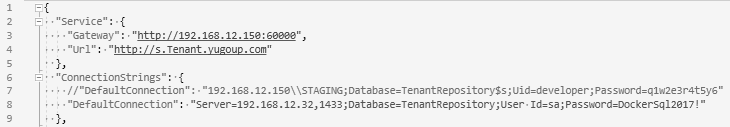
\includegraphics[width=0.9\linewidth]{Cap6/TenantConnectionString.png}
\caption{\textit{Connection String} da Base de Dados}
\label{Fig:Fig80}
\end{figure}

\begin{figure}[hbt!]
\centering
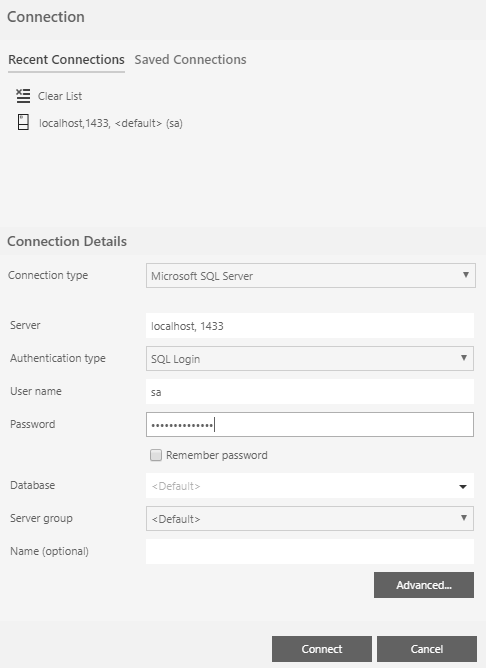
\includegraphics[width=0.4\linewidth]{Cap6/MSSQLServerTenantRepository.png}
\caption{Conexão ao serviço de base de dados pelo \textbf{Azure Data Studio}}
\label{Fig:Fig81}
\end{figure}

\hspace{1cm}A imagem do serviço foi depois publicada com a \textit{tag} \textbf{t-yugoup-tenant} e posteriormente foi lançado um \textit{container} com o projeto da \textbf{Web API} que mais tarde foi acedido pelo \textit{browser}.

\subsection{Resultados}

\hspace{1cm}A apresentação dos resultados dos testes e da análise estática vai ser o produto final da \textit{pipeline} de testes automatizada. 

\subsubsection{Apresentação dos resultados dos testes}

\hspace{1cm}A apresentação dos resultados dos testes no \textbf{Jenkins} é feita com um gráfico. Este gráfico contém o número de testes -- \textit{Passed, Failed e Skipped} -- no eixo dos \textbf{y} e o número da \textit{build} no eixo dos \textbf{x}. 
Na figura \ref{Fig:Fig70} são apresentados os resultados dos testes, na sua maioria, por um tom de cinza intermédio.

\begin{figure}[hbt!]
\centering
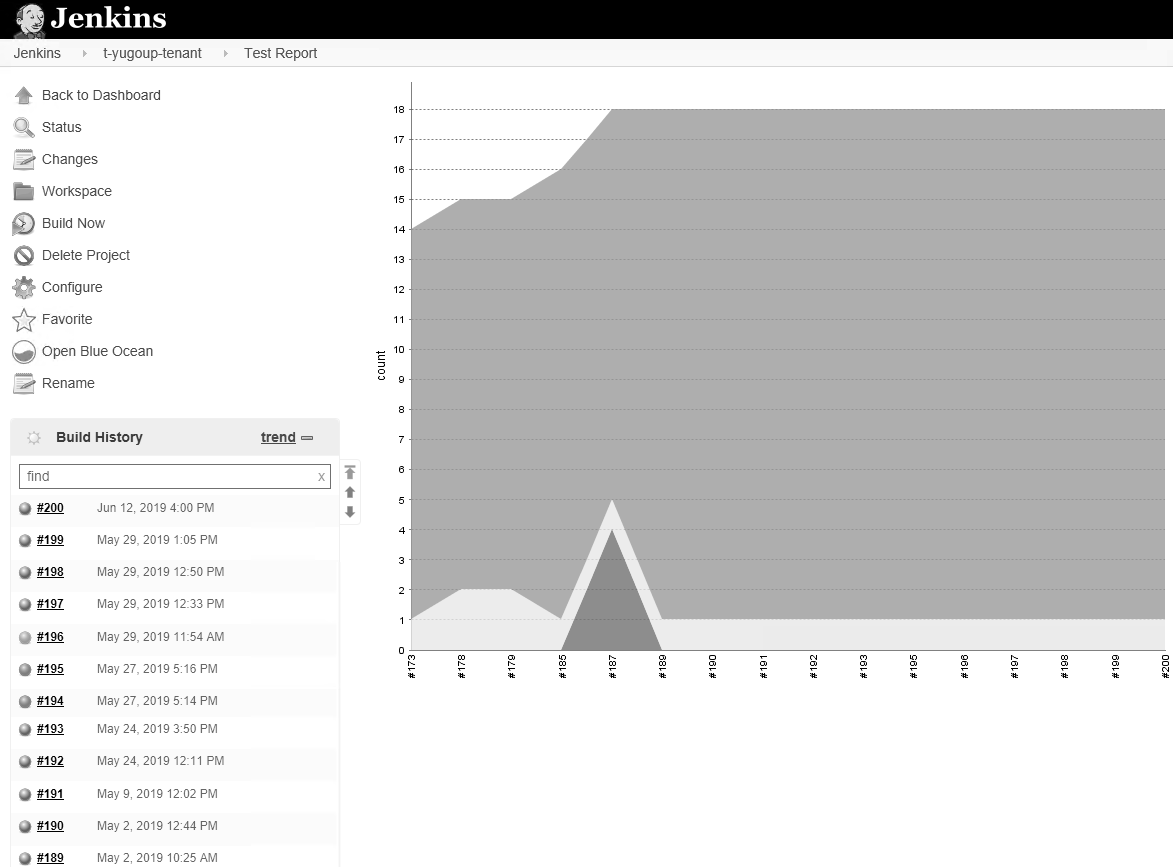
\includegraphics[width=0.9\linewidth]{Cap6/TenantTestResults.png}
\caption{Resultado dos testes}
\label{Fig:Fig70}
\end{figure}

Quer isto dizer que grande parte dos testes são executados com sucesso. Na \textit{build} número 187 foi introduzida a análise aos quatro testes de integração, dois dos quais com testes de performance, cujo resultado inicial da execução não foi de encontro ao esperado, sendo possível ver pela cor cinza escuro. No entanto duas \textit{builds} depois (189) os testes foram compilados e executados com sucesso, o que resultou numa subida no número total de testes \textit{Passed}. Para ser vista a representação dos testes \textit{Skipped} foi criado, a título de exemplo, um teste unitário em \textbf{MSTest} com o atributo \textbf{Skip} -- representado a cinza claro -- para ser conhecida a sua interpretação gráfica. 

\hspace{1cm}No total, o serviço do \textbf{Tenant} contabiliza dezoito testes. Destes dezoito testes, um é passado à frente (\textit{Skipped}). Quatro desses dezoito testes são testes feitos à integração dos \textit{endpoints} da plataforma e dois desses quatro testes são testados em termos de performance. Os restantes treze testes são testes unitários, feitos às camadas de manipulação e tratamento de dados da plataforma.

\subsubsection{Resultados da análise estática}

\hspace{1cm}A análise estática apresentou um conjunto alertas relativos a falhas de segurança, \textit{bugs}, \textit{Code Smells} e vulnerabilidades dentro da plataforma, no entanto o \textbf{quality gate} foi positivo, como é possível verficar-se na figura \ref{Fig:Fig71}.

\hspace{1cm}Foram identificados 27 \textit{Bugs}, 37 \textit{Vulnerabilities}, 634 \textit{code smells} e 193 \textit{Security Hotspots}. Em termos de gravidade, foram identificados 5 \textit{Issues} do tipo \textit{Blocker}, 198 do tipo \textit{Minor}, 105 do tipo \textit{Critical}, 385 do tipo \textit{Major} e 5 do tipo \textit{Info}. Toda a informação acerca dos \textit{Issues} identificados pela análise estática do \textbf{Sonarqube} é descrita em detalhe na documentação oficial \cite{sonarqubetooldocs}.

\begin{figure}[hbt!]
\centering
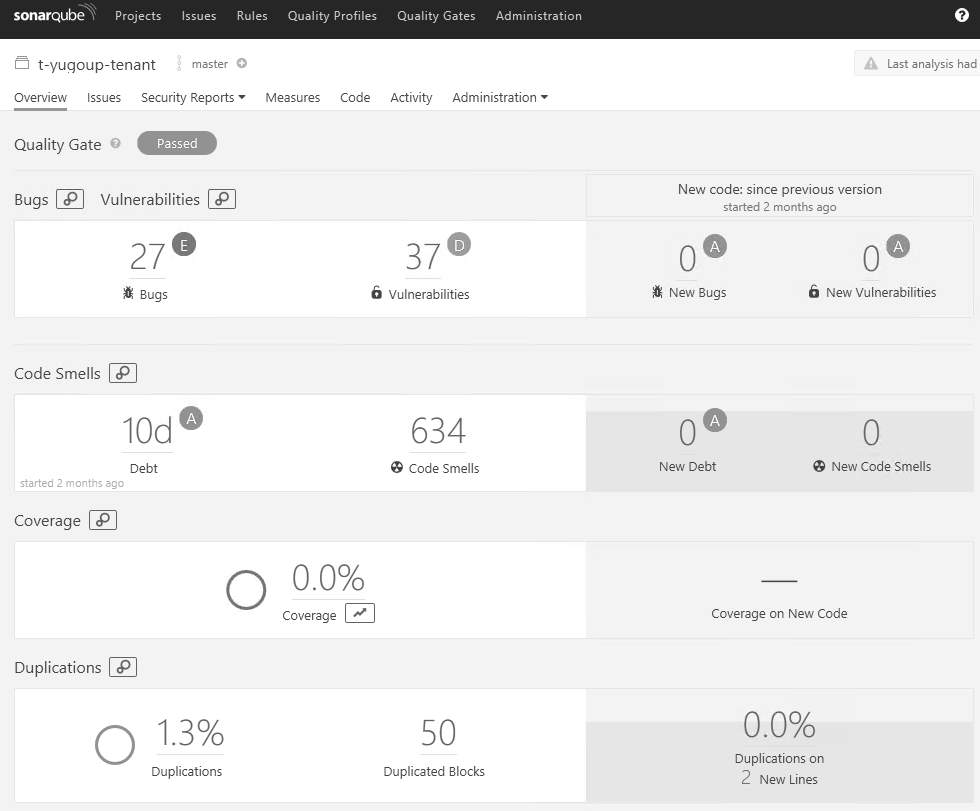
\includegraphics[width=0.9\linewidth]{Cap6/TenantStaticAnalysis.png}
\caption{\textit{Overview} da análise estática}
\label{Fig:Fig71}
\end{figure}

\subsection{Considerações}

\hspace{1cm}Após a conclusão da execução da \textit{pipeline} verificamos que o serviço do \textit{Tenant} está validado com uma bateria de testes e com a análise estática. Numa primeira fase, depois da junção de todos os projetos numa pasta final, é executada análise estática. Inicialmente a análise estática iria ser executada contra o serviço do \textit{Tenant}. No entanto, apesar da \textit{build} ser feita apenas ao serviço que pretendíamos analisar inicialmente, todos os projetos que estão dependentes do serviço vão ser analisados. Como muitos projetos dependem, direta ou indiretamente, do serviço do \textit{Tenant} vamos ter a plataforma \textbf{da Yugoup} analisada por completo. Apesar de ir contra o objetivo inicial, a análise estática faz mais do que aquilo que inicialmente foi estabelecido. A análise estática é fundamentalmente uma análise léxica e sintática do código desenvolvido pela equipa da Yugoup. É possível afirmar também que a análise estática pode incorporar análise semântica tendo em conta o contexto do negócio. Do ponto de vista funcional, o \textbf{Sonarqube} é incluído na \textit{pipeline} porque é fundamental que todo o código seja revisto e analisado de acordo com as boas práticas de programação e para que seja verificado que não existem variáveis, métodos ou chamadas de funções não implementados ou não utilizados dentro da plataforma.

\hspace{1cm}A execução dos testes unitários é importante do ponto de vista semântico e de compilação. Com os testes unitários, são feitas verificações ao modelo da aplicação que é testado de acordo com um conjunto de especificações, tendo em conta as funcionalidades implementadas, as quais foram pedidas com regras pelo \textit{business}. Os testes unitários também procuram testar se essas mesmas regras são aplicadas e se os resultados obtidos vão de encontro aos resultados esperados.

\hspace{1cm}Os testes de integração e performance são utilizados para testar a integração entre serviços através da comunicação com \textit{endpoints} na máquina de \textit{staging}. Junto com testes de integração, são aproveitados os tempos de resposta, tempos esses que são -- após execução dos testes -- dados como testes de performance.

\begin{figure}[hbt!]
\centering
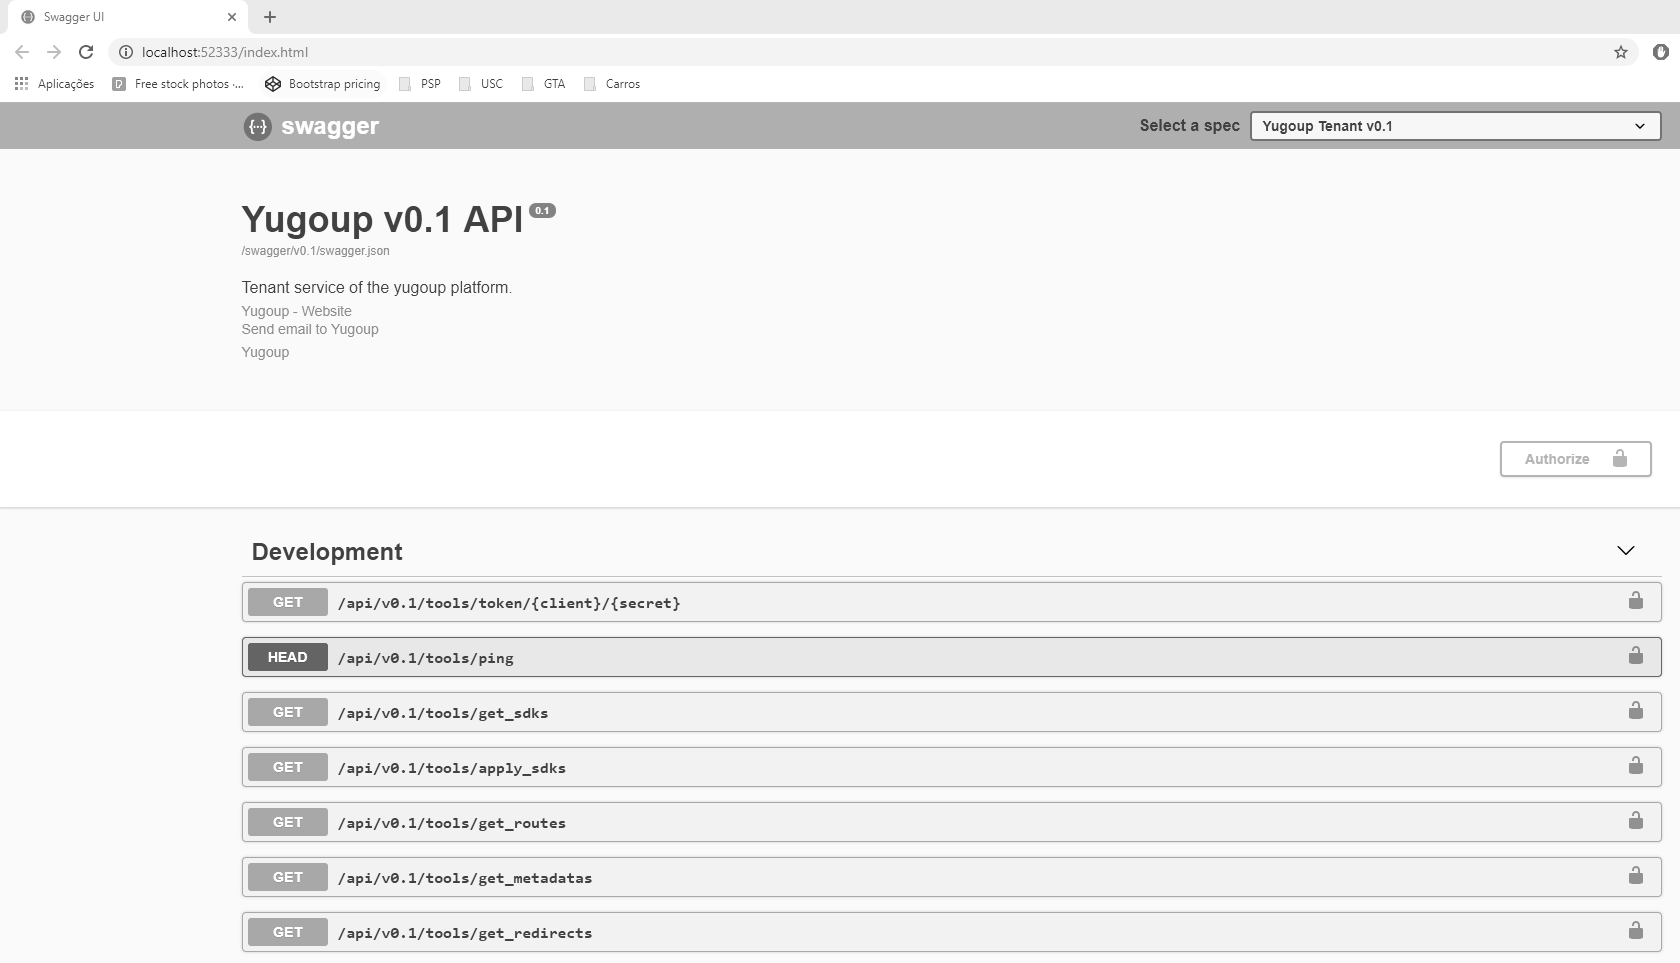
\includegraphics[width=0.9\linewidth]{Cap6/TenantScreenShot.png}
\caption{\textit{Screenshot} do serviço \textit{Tenant} executado a partir do IDE}
\label{Fig:Fig83}
\end{figure}

\begin{figure}[hbt!]
\centering
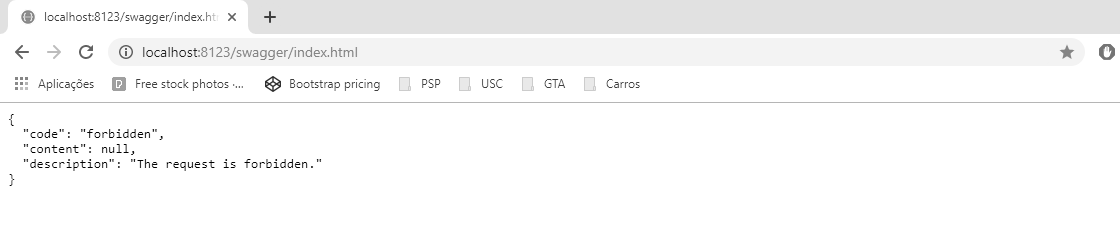
\includegraphics[width=0.9\linewidth]{Cap6/TenantServiceNotRespondingScreenShot.png}
\caption{\textit{Screenshot} do serviço \textit{Tenant} executado a partir da imagem \textbf{Docker}}
\label{Fig:Fig84}
\end{figure}

\hspace{1cm}O \textit{Tenant} funciona como esperado quando executado a partir do ambiente integrado de desenvolvimento (\ref{Fig:Fig83}). Mesmo com a base de dados de \textbf{SQL Server} servida a partir do \textit{container}. Por outro lado, o comportamento do serviço \textit{Tenant}, quando executado a partir da imagem gerada anteriormente através do \textit{Dockerfile} -- que pode ser visualizado nas figuras \ref{Fig:Fig77}, \ref{Fig:Fig78} e \ref{Fig:Fig79} -- é diferente  (\ref{Fig:Fig84}) do esperado. O problema apresentado é uma medida de segurança, a qual pode ser descativada, que foi implementada para proibir interações que não estejam configuradas ou esperadas. Esta medida de segurança usa-se para colocar um serviço por detrás de um \textit{Gateway}, o qual é o único a ter acesso a essa API. A configuração garante que apenas e só -- e só mesmo -- o serviço \textit{Gateway} consegue comunicar com esses serviços. Este mecanismo apresenta também a vantagem de prevenir \textbf{DDoS} pois, em termos de \textit{stack} de chamada, faz com que o pedido falhe imediatamente sem ocupar grande quantidade de recursos.

\section{Integração de sistemas de visualização}
\label{Ch:CapExemplo}

\hspace{1cm}Como forma de obter feedback mais rápido acerca do resultado da \textit{pipeline} surgiu a necessidade de implementação de um sistema de visualização integrado no ciclo de desenvolvimento e teste de software. O principal objetivo da integração deste sistema de visualização seria a colocação do estado de uma \textit{build} num monitor LCD disponibilizado pela empresa. O sistema servirá para notificar os \textit{developers} acerca do estado das \textit{builds} e estará ligado, em rede local, à máquina de  \textit{staging} que, por sua vez, conta com uma instância do \textit{Jenkins} pronta a executar um conjunto de \textit{Jobs}.

\subsection{Sistema de visualização}

As especificações do sistema, em termos de requisitos funcionais, seriam as seguintes: 

\begin{itemize}
  \item O sistema deve apresentar o resultado final de uma \textit{build};
  \item O sistema deve notificar os \textit{developers};
  \item O sistema deve utilizar o LCD disponibilizado pela empresa;
  \item O sistema deve utilizar um Raspberry PI;
  \item O sistema deve estar conectado à rede local;
\end{itemize}

\hspace{1cm}Para além da monitorização -- quase instantânea -- dos \textit{jobs}, o sistema de visualização estará disponível via FTP \textit{(File Transfer Protocol)}. Isto permitirá a inclusão de um conjunto de ficheiros, como os ficheiros com as credenciais de acesso à máquina de \textit{staging}, para facilitar a conexão ao sistema central.

\subsection{Integração do sistema de visualização}

\hspace{1cm}Para a integração de um sistema idêntico de visualização em rede -- local ou online -- é necessário que o sistema central conte com:

\begin{itemize}
  \item Uma instância do \textbf{\textit{Jenkins}};
  \item O \textit{Plugin} \textbf{\textit{Build Monitor}};
  \item Um \textbf{\textit{Job}};
\end{itemize}

\hspace{1cm}Para a integração do sistema de visualização vão ser necessários:

\begin{itemize}
  \item Um \textbf{\textit{Raspberry PI}}, com o respetivo carregador;
  \item Um \textbf{\textit{SD Card}} com, pelo menos, 8GB de memória;
  \item Um teclado;
  \item Um rato ótico (opcional);
  \item Um monitor, como referido anteriormente;
  \item Um cabo de rede;
  \item Um cabo HDMI;
\end{itemize}

\subsection{Instalação do sistema de visualização}

\hspace{1cm}O primeiro passo para que seja possível integrar o sistema de visualização no ciclo de desenvolvimento de software é a formatação do cartão de memória que irá conter o sistema operativo do mini-computador, o \textbf{\textit{Raspberry PI}}. Para a formatação do \textbf{\textit{SD Card}} existem vários softwares disponíveis mas, neste caso, foi utilizado o software \textbf{\textit{SD Card Formatter}}.

\hspace{1cm}De seguida, procede-se à instalação do sistema operativo no \textbf{\textit{SD Card}} pré-formatado. No site oficial da \textbf{Raspberry} são disponibilizados vários sistemas operativos, juntamente com um instalador de sistemas operativos, na secção de downloads. Neste caso, foi utilizado o \textbf{\textit{NOOBS}} (\textit{New Out-of-the Box Software}), que é um instalador de sistemas operativos \textit{user-friendly}.

\subsection{Configuração do sistema de visualização}

\hspace{1cm}Para proceder à configuração do sistema de visualização certifica-se, primeiramente, que o dispositivo contém uma fonte de alimentação com a potência adequada. Após essa verificação, conecta-se o teclado, o rato (caso se disponha de um), o cabo HDMI e o cabo de rede. Antes de se proceder à primeira execução do dispositivo, insere-se o \textbf{\textit{SD Card}} na parte inferior do \textbf{\textit{Raspberry PI}} com o instalador de sistemas operativos, ou com a imagem do sistema operativo que vai ser utilizado. Só depois de se completar os passos anteriores é ligado o dispositivo à corrente. Se todos os passos tiverem sido devidamente executados, o sistema de configuração do dispositivo deve arrancar dentro de alguns momentos.

\hspace{1cm}A primeira vez que o \textbf{\textit{Raspberry PI}} arranca é mais demorada e requer a instalação dos módulos e componentes do sistema. Dito isto, quanto mais rápida for a conexão à rede, mais rápido será o download do sistema operativo e dos seus módulos e, consequentemente, mais rápida será a configuração do dispositivo.


\hspace{1cm}Após a instalação dos módulos e do sistema operativo, o dispositivo terá de ser reiniciado para que sejam aplicadas as alterações. Neste caso, em particular, foi instalado o \textbf{raspbian}, o sistema operativo desenvolvido pela marca \textbf{\textit{Raspberry PI}}, que é baseado no \textbf{Debian}, um sistema operativo \textit{open source}. Este sistema operativo apresenta uma \textit{Graphical User Interface} semelhante ao ambiente de trabalho, \textit{user-friendly}, dos seus homólogos mais conhecidos -- \textbf{Windows} e \textbf{Ubuntu} -- que facilita a sua aprendizagem (\ref{Fig:Fig4}).

\begin{figure}
\centering
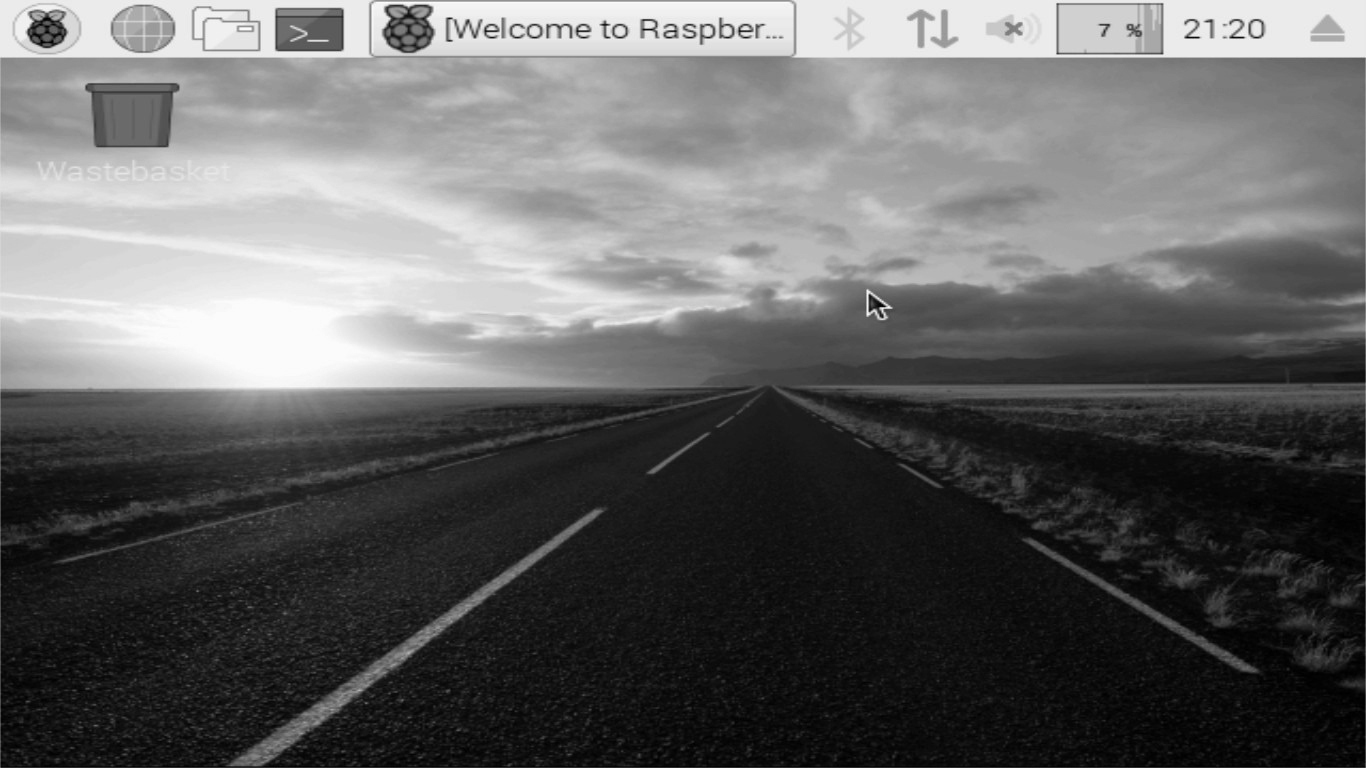
\includegraphics[width=0.5\linewidth]{Cap8/RaspberryPiWorkEnvironment.png}
\caption{Ambiente de trabalho do \textit{rasbpian}}
\label{Fig:Fig4}
\end{figure}

\subsection{Apresentação do estado das builds}

\hspace{1cm}O estado das builds, que será mostrado no LCD, fará uso do \textit{plugin} \textbf{\textit{Build Monitor}} que foi previamente instalado na instância do \textbf{Jenkins} da máquina de \textit{staging} que a empresa disponibilizou. Tendo em conta que um dos pressupostos para a implementação deste sistema passava pelo seu funcionamento em rede local, é necessário aceder ao endereço de IP da máquina de \textit{staging}.

\hspace{1cm}Para ser possível criar a \textit{view} do \textbf{\textit{Build Monitor}}, na página principal do orquestrador de processos, clica-se na \textit{tab} que contém um sinal ``+'', por cima dos \textit{jobs}, seleciona-se o \textit{radiobutton} com a opção \textit{``Build Monitor View''} e atribui-se um nome (\ref{Fig:Fig5}).  

\begin{figure}
\centering
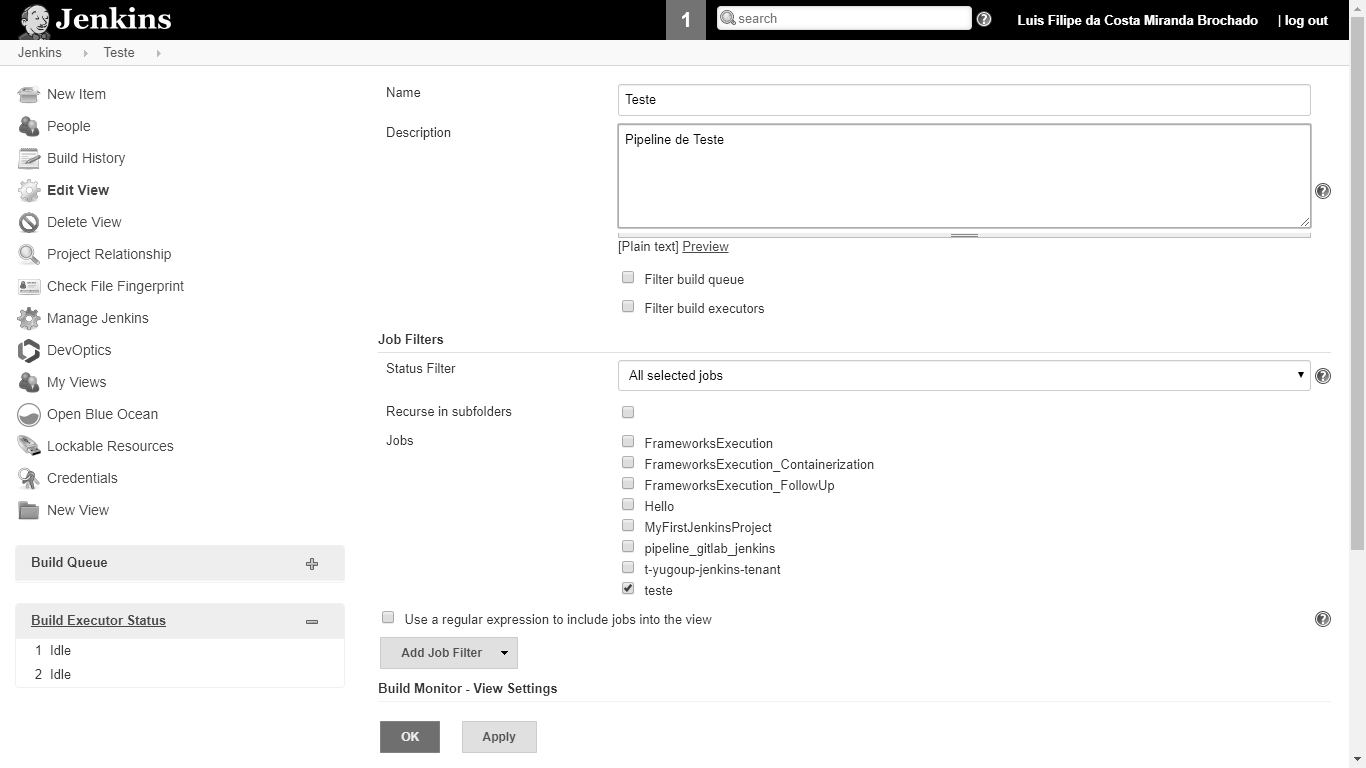
\includegraphics[width=0.9\linewidth]{Cap8/BuildMonitorConfig.png}
\caption{Configuração da \textit{view}}
\label{Fig:Fig5}
\end{figure}

\hspace{1cm}Já dentro do painel de configuração da \textit{view} podemo ser definidos um conjunto de critérios. Desde uma descrição, um filtro por estado do \textit{job}, o nome do último \textit{job}, o seu tempo de execução, etc. Neste caso, será apenas testado o seu funcionamento, portanto, seleciona-se o \textit{job} "teste" que foi anteriormente criado com esse propóstito (\ref{Fig:Fig6}).

\begin{figure}
\centering
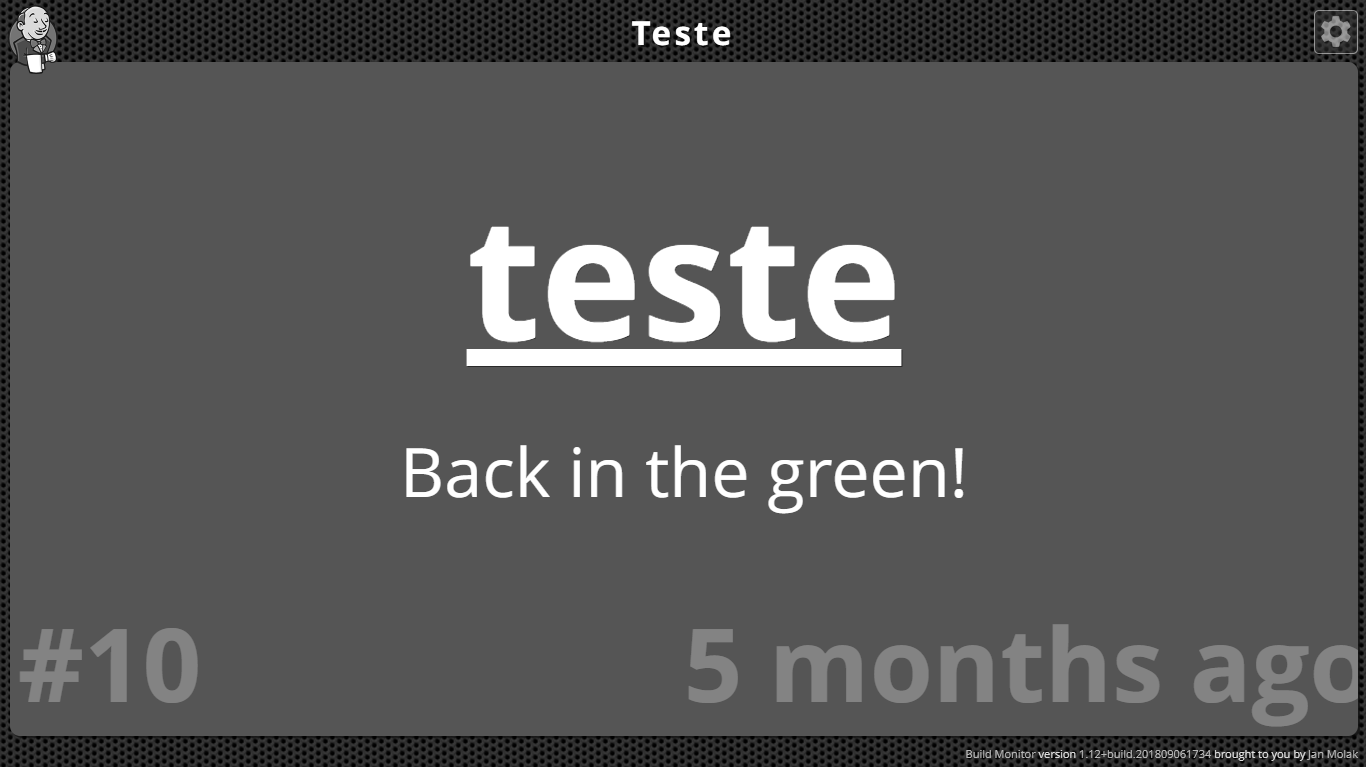
\includegraphics[width=0.9\linewidth]{Cap8/BuildMonitorView.png}
\caption{Estado do \textit{job}}
\label{Fig:Fig6}
\end{figure}

\hspace{1cm}Tendo em conta que o objetivo da instalação de um sistema deste tipo é a sua mostragem constante no ecrã, para efeitos de monitorização, será necessária uma configuração adicional ao \textbf{Raspberry PI} para que o dispositivo não entre em hibernação. Para tal, após alguma pesquisa, verificou-se que existiam um conjunto de soluções nos fóruns oficiais da \textbf{RasbperryPI} nos \textit{posts} \textit{\cite{rasbperryPIFix}} e \textit{\cite{rasbperryPIFix2}}. A solução passou por alterar algumas linhas nos ficheiros de configuração do sistema operativo.

\subsection{Pontos críticos}

\hspace{1cm}A utilização de um pequeno dispositivo com baixa capacidade de computação foi suficiente para criar algum \textit{engagement} entre a equipa de desenvolvimento. Contudo, caso se pretenda um dispositivo com melhor performance, devem ter-se em atenção alguns aspetos. Em termos comparativos, o dispositivo utilizado tem um conjunto de sucessores com performance superior. A versão do \textbf{\textit{Raspberry PI}} \cite{rasbperryPIModel3}, segundo o website da marca, conta com as seguintes especificações base:

\begin{itemize}
 \item Quad Core 1.2GHz Broadcom BCM2837 64bit CPU
1GB RAM;
 \item BCM43438 wireless LAN and Bluetooth Low Energy (BLE) on board;
 \item 100 Base Ethernet;
 \item 40-pin extended GPIO;
 \item 4 USB 2 ports;
 \item 4 Pole stereo output and composite video port;
 \item Full size HDMI;
 \item CSI camera port for connecting a Raspberry Pi camera;
 \item DSI display port for connecting a Raspberry Pi touchscreen display;
 \item Micro SD port for loading your operating system and storing data;
 \item Upgraded switched Micro USB power source up to 2.5A;
\end{itemize}

\hspace{1cm}Apesar de existirem dispositivos com performance algo superior, um dispositivo semelhante ao utilizado é mais do que suficiente para o tipo de trabalho que foi designado.

\hspace{1cm}Um dos fatores que contribui imenso para a performance do dispositivo, para além da velocidade de conexão à internet, é o tipo de \textbf{\textit{SD Card}} utilizado. Para melhor performance, recomenda-se a utilização de um cartão classe 10 (C-10) de 16 ou 32GB. A capacidade do cartão não afeta diretamente o tempo de resposta. Contudo, o tempo de leitura e o tempo de escrita podem diferir entre cartões da mesma classe. Na tabela apresenta-se a performance do mesmo \textbf{\textit{Raspberry PI}} com cartões diferentes. Os tempos apresentados serviram para medir o tempo desde que o dispositivo inicia até que está 100\% operacional.

\begin{center}
\begin{tabular}{ |c||p{3cm}|p{3cm}|  }
 \hline
 \multicolumn{3}{|c|}{Tempos de espera até iniciar o sistema operativo} \\
 \hline
 Tentativa & \textit{SD Card} 16GB & \textit{SD Card} 32GB\\
 \hline
 $t_{1}$ & 1:55.84 (min) & 1:31:56 (min)\\
 $t_{2}$ & 1:55.30 (min) & 1:26:67 (min)\\
 $t_{3}$ & 1:55.64 (min) & 1:34:15 (min)\\
 $t_{4}$ & 1:52.33 (min) & 1:30:10 (min)\\
 $t_{5}$ & 1:56.32 (min) & 1:28:75 (min)\\
 $t_{6}$ & 1:58.67 (min) & 1:35:18 (min)\\
 $t_{7}$ & 2:00.67 (min) & 1:35:43 (min)\\
 $t_{8}$ & 1:55.90 (min) & 1:35:57 (min)\\
 $t_{9}$ & 1:57.55 (min) & 1:37:41 (min)\\
  \hline
 Média (min) & 1:55.46 (min) & 1:32.76 (min)\\
 \hline
\end{tabular}
\end{center}

\hspace{1cm}O primeiro cartão testado com 16GB de capacidade tinha, segundo as especificações, velocidade de leitura na ordem dos 18.6 MB/s e velocidade de escrita na ordem dos 10.2 MB/s. Já o segundo cartão testado tinha 32GB de capacidade e, segundo as especificações, contava com velocidade de leitura e de escrita bastante superiores, 95 MB/s e 25 MB/s, respetivamente.  

\hspace{1cm}Pode concluir-se que, por si só, a utilização de um \textit{SD Card} com melhor performance apresenta melhores resultados para este caso, onde o objetivo foi medir o tempo de espera até o sistema operativo do dispositivo estar \textit{"fully operational"}. Como é evidente, este intervalo de tempo não contabiliza a abertura do \textit{Browser} e a creditação no \textit{Jenkins} para a apresentação do estado das \textit{builds}. Contudo, é importante referir que o \textit{SD Card} cuja velocidade (estimada) de leitura e escrita se diz de melhor performance foi mais rápido, em média, 23.30 segundos do que o \textit{SD Card} disponibilizado pela empresa. Este \textit{upgrade} representa uma melhoria de 20.3\% no que diz respeito à demora ao iniciar o sistema operativo para o mesmo dispositivo.

\hspace{1cm}Como referido anteriormente, este dispositivo -- cedido pela empresa -- é mais do que suficiente para a função que está a desempenhar. No entanto, caso se pretenda um dispositivo com melhor \textit{performance}, existem no mercado várias soluções que podem ser estudadas. Existe por exemplo a versão mais recente do dispositivo, o {\textbf{Raspberry PI model 3 b+ \cite{rasbperryPIModel3bplus}}} cuja ficha técnica apresenta, segundo a marca, especificações base superiores.

